%%%%%%%%%%%%%%%%%%%%%%%%%%%%%%%%%%%%%%%%%%%%%%%%%%%%%%%%%%%%%%%%%%%%%%%%%%%%%
%%% LaTeX-Rahmen fuer das Erstellen von Masterarbeiten
%%%%%%%%%%%%%%%%%%%%%%%%%%%%%%%%%%%%%%%%%%%%%%%%%%%%%%%%%%%%%%%%%%%%%%%%%%%%%

%%%%%%%%%%%%%%%%%%%%%%%%%%%%%%%%%%%%%%%%%%%%%%%%%%%%%%%%%%%%%%%%%%%%%%%%%%%%%
%%% allgemeine Einstellungen
%%%%%%%%%%%%%%%%%%%%%%%%%%%%%%%%%%%%%%%%%%%%%%%%%%%%%%%%%%%%%%%%%%%%%%%%%%%%%

\documentclass[12pt,a4paper]{report}
%\usepackage[utf8]{inputenc}

\usepackage{amsmath}
%\usepackage[scaled=0.92]{helvet}
\usepackage{tikz}
\usetikzlibrary{shapes.geometric, arrows, calc}

% Definition der Styles
\tikzstyle{startstop} = [rectangle, rounded corners, minimum width=3cm, minimum height=1cm,text centered, draw=black, fill=red!30]
\tikzstyle{process} = [rectangle, minimum width=3cm, minimum height=1cm, text centered, draw=black, fill=blue!10]
\tikzstyle{arrow} = [thick,->,>=stealth]
\tikzstyle{io} = [trapezium, trapezium left angle=70, trapezium right angle=110, minimum width=3cm, minimum height=1cm, text centered, draw=black, fill=blue!30]
\tikzstyle{decision} = [diamond, minimum width=3cm, minimum height=1cm, text centered, draw=black, fill=green!30]
\tikzstyle{subroutine} = [rectangle, double, minimum width=4cm, minimum height=1cm, text centered, draw=black, fill=orange!10]
\usepackage[scaled=1.1]{nimbusmononarrow}
%\usepackage[T1]{fontenc}

\usepackage{microtype} %Ermöglicht Blocksatz durch minimale Veränderung der Buchstabenbreite
\usepackage{noto}
\usepackage{subcaption}
\usepackage{cite}
\usepackage{eurosym}
\usepackage[english,ngerman]{babel}
\usepackage{bibgerm}
\usepackage{graphics, graphicx}
\usepackage{wrapfig}
\usepackage[margin=10pt,font=small,labelfont=bf]{caption}
\usepackage{sistyle}
\usepackage{latexsym}
\usepackage{hyperref}
\usepackage{csquotes}
\usepackage[textwidth=14cm,textheight=22cm]{geometry}
\usepackage{url}
\usepackage{caption}
\usepackage{float}
\usepackage{tabularx}
\usepackage{pdfpages} 
\usepackage{pdflscape}
\usepackage[toc,page]{appendix}


\usepackage{titlesec}
\titleformat{\chapter}[hang] % Kapitelüberschrift in einer Zeile
{\normalfont\Huge\bfseries} % Schriftart, Größe, fett
{\thechapter\quad}          % Kapitelnummer mit Abstand
{0pt}                       % Abstand zwischen Nummer und Text
{}                          % Kein zusätzlicher Text (wie "Kapitel")

% Abstand vor und nach Kapitelüberschrift ändern (optional):
\titlespacing*{\chapter}{0pt}{*3}{*2}

%\footskip 2cm
%\parskip 0.5ex plus 0.1ex minus 0.1ex
%\parindent0pt
\usepackage{setspace}
\onehalfspacing   

%Numerierungstiefe
\setcounter{secnumdepth}{3}
%Inhaltsverzeichnis-Tiefe
\setcounter{tocdepth}{3}

% Hurenkinder und Schusterjungen verhindern
% http://projekte.dante.de/DanteFAQ/Silbentrennung -- link deprecated!
\clubpenalty = 10000 % schließt Schusterjungen aus (Seitenumbruch nach der ersten Zeile eines neuen Absatzes)
\widowpenalty = 10000 % schließt Hurenkinder aus (die letzte Zeile eines Absatzes steht auf einer neuen Seite)
\displaywidowpenalty=10000


% Kann nach persönlichem Geschmack verändert werden.
%\usepackage{fancyhdr}
%\pagestyle{fancy}
%\fancyhead[LO,RE]{\textsl{\nouppercase{\leftmark}}}
%\fancyhead[LE,RO]{\thepage}
%\fancyfoot{}

%\fancyhead[LE,RO]{\textsl{\rightmark}}


% Kommentar-Style zum Einfügen von To-Do's Befehle: \todo , \note und \listoftodos
\usepackage[textsize=footnotesize,textwidth=0.8in]{todonotes} % Kommentare einschalten
%\usepackage[disable]{todonotes} % Kommentarausgabe ausschalten
\setlength{\emergencystretch}{0.8in} % Abstand vom Rand
\newcommand{\note}{\todo[inline,color=yellow,caption={}]} %Notiz über volle Seitenbreite

%Blockschaltbilder
\usepackage{tikz}
\usetikzlibrary{positioning, arrows.meta, shapes.geometric}

\tikzset{
	block/.style = {draw, rectangle, minimum height=2em, minimum width=4em},
	arrow/.style = {->, >=Stealth}
}
%%%%%%%%%%%%%%%%%%%%%%%%%%%%%%%%%%%%%%%%%%%%%%%%%%%%%%%%%%%%%%%%%%%%%%%%%
% kopf und fußzeile
\usepackage[headsepline, footsepline, plainheadsepline, plainfootsepline]{scrlayer-scrpage}		% linie aktivieren für "headings" und "plain" seiten
%\automark{chapter}		% aktivieren das "chapter" und "section" oeben angezeigt werden kann
%\automark*{section}

\setlength{\headheight}{35pt}			% header abstand
\setlength{\footheight}{\baselineskip}	% footer abstand

\clearpairofpagestyles

% Der "*" macht, dass hier konfigurierte Einstellungen auch für "plain"-Seiten gelten
%\ihead*{\vspace*{-0.0cm}\includegraphics[height=1cm, width=0.3\textwidth, keepaspectratio, angle=0]{\firmenlogo}}	%pdf firmenlogo etwas runtersetzen, da komisch formatiert
\chead{\normalfont \headmark}		% "chapter" und "section" oben mittig anzeigen
\ohead*{
\includegraphics[height=1cm, angle=0]{figures/dhbwlogo.png}}	% DHBW Logo

\ifoot*{\scriptsize \normalfont Autoren: \autor \ | \ \autorzwei}	% Autoren hintereinander in einer Zeile (Links)
%\cfoot*{}  % Mitte bleibt leer, Datum entfernt
\ofoot*{\pagemark} % Seitenzahl (Rechts)

%%%%%%%%%%%%%%%%%%%%%%%%%%%%%%%%%%%%%%%%%%%%%%%%%%%%%%%%%%%%%%%%%%%%%%%%%
%TODO: create variables and implement syntax like \art{T1000}
\newcommand{\art}{Studienarbeit T3200} %feminin
\newcommand{\titel}{Cognitive Robotics}
\newcommand{\untertitel}{}

\newcommand{\studiengang}{Elektrotechnik}
\newcommand{\studienfach}{Elektrotechnik} %Wird nur für Bachelordeckblatt benötigt.
\newcommand{\fachrichtung}{Elektronik} 
\newcommand{\hochschule}{Dualen Hochschule Stuttgart} %An der ...
\newcommand{\campus}{Campus Horb}

\newcommand{\autor}{Luis Magnus Thiel}
\newcommand{\strassehausnr}{Hugo-Bertsch-Straße 15}
\newcommand{\plzwohnort}{72459 Albstadt}

\newcommand{\autorzwei}{Adrian Sommer}
\newcommand{\strassehausnrzwei}{Hechinger Straße 40}
\newcommand{\plzwohnortzwei}{72336 Balingen}

\newcommand{\jahrgang}{TET2023}
\newcommand{\matrikelnr}{8616207}
\newcommand{\matrikelnrzwei}{9519924}
\newcommand{\kurs}{ET2023} % Nicht verwendet
\newcommand{\bearbeitungszeitraum}{02. März 2026 bis 22. Juni 2026}
\newcommand{\betreuer}{Norman Bläse (Mercedes-Benz)}
\newcommand{\ausbildungsleiter}{} % Nicht verwendet
\newcommand{\gutachter}{Musterbetreuer 2} % Nicht verwendet

\newcommand{\dateiname}{Studienarbeit T3200} % Nicht verwendet
\newcommand{\abgabeort}{Horb am Neckar}
\newcommand{\firma}{ASSA ABLOY Sicherheitstechnik GmbH}
\newcommand{\firmenstrasse}{Bildstockstraße 20}
\newcommand{\firmenort}{72458 Albstadt}
\newcommand{\firmenlogo}{figures/assaabloy_logo.jpg}
\newcommand{\firmazwei}{Groz-Beckert KG}
\newcommand{\firmenstrassezwei}{Parkweg 2}
\newcommand{\firmenortzwei}{72458 Albstadt}
\newcommand{\csharp}{C\#}

\newcommand{\ladeliteratur}{
	\addbibresource{Literatur.bib}
	%\addbibresource{WeitereLiteratur.bib}

}
%%%%%%%%%%%%%%%%%%%%%%%%%%%%%%%%%%%%%%%%%%%%%%%%%%%%%%%%%%%%%%%%%%%%%%%%%
\begin{document}

%%%%%%%%%%%%%%%%%%%%%%%%%%%%%%%%%%%%%%%%%%%%%%%%%%%%%%%%%%%%%%%%%%%%%%%%%%%%
%%% hier steht die neue Titelseite 
%%%%%%%%%%%%%%%%%%%%%%%%%%%%%%%%%%%%%%%%%%%%%%%%%%%%%%%%%%%%%%%%%%%%%%%%%%%%
\begin{titlepage}
	
	\thispagestyle{plain}
	\renewcommand*{\pagemark}{} % Unterdrückt die Ausgabe der Seitenzahl (Lokal für diese Umgebung)
	\ifoot*{}
	\vspace{-10pt}
	\begin{center}
		
		\begin{LARGE}
			\titel
			\\		
			\vspace{14pt}
		\end{LARGE}
		\begin{LARGE}
			\art\\
			\vspace{16pt}
		\end{LARGE}
		\begin{LARGE}
			\untertitel	
		\end{LARGE}
	\end{center}
	
	\begin{center}
		Studiengang \studienfach\\
		%Fachrichtung \fachrichtung
		
		An der \hochschule \\ \campus\\
	\end{center}
	
	\let\stretchbuffer\arraystretch % buffer \arraystretch to restore later
	\renewcommand{\arraystretch}{1.25} % make table spacing same as line spacing
	\begin{table}[b!]
		\normalsize
		\begin{tabularx}{\textwidth}{lXX} % 3 Spalten: 1x linksbündig (Labels), 2x für die Autoren
			% NEU: "Eingereicht von:" über den Autoren-Spalten (2 Spalten, linksbündig)
			\multicolumn{1}{l}{\textbf{Eingereicht von:}} & \multicolumn{2}{l}{} \\
			\\[-0.5em] 
			
			\textbf{Name:} 			& \autor 				& \autorzwei \\
			\textbf{Matrikelnr.:} 	& \matrikelnr 			& \matrikelnrzwei \\
			\textbf{Straße, Nr.:} 	& \strassehausnr 		& \strassehausnrzwei \\
			\textbf{PLZ, Ort:} 		& \plzwohnort 			& \plzwohnortzwei \\
			\\[1cm]
			% Firmeninformationen in separaten Spalten
			\textbf{Partner:} 	    & \firma 				& \firmazwei \\
			\textbf{Adresse:} 	    & \firmenstrasse 		& \firmenstrassezwei \\
			\textbf{Ort:} 	        & \firmenort 			& \firmenortzwei \\
			\\[1cm]
			
			% Zusätzliche Informationen über volle Breite
			\multicolumn{3}{l}{\textbf{Studienjahrgang:} \jahrgang} \\
			\multicolumn{3}{l}{\textbf{Bearbeitungszeitraum:} \bearbeitungszeitraum} \\
			\multicolumn{3}{l}{\textbf{Betreuer:} \betreuer} \\
		\end{tabularx}
	\end{table}
	\renewcommand{\arraystretch}{\stretchbuffer} % restore \arraystretch
	%\clearpage
\end{titlepage}
%%%%%%%%%%%%%%%%%%%%%%%%%%%%%%%%%%%%%%%%%%%%%%%%%%%%%%%%%%%%%%%%%%%%%%%%%%%%

\pagenumbering{roman}
\setcounter{page}{1}

%%%%%%%%%%%%%%%%%%%%%%%%%%%%%%%%%%%%%%%%%%%%%%%%%%%%%%%%%%%%%%%%%%%%%%%%%%%%
%%% Kurzzusammenfassung
%%%%%%%%%%%%%%%%%%%%%%%%%%%%%%%%%%%%%%%%%%%%%%%%%%%%%%%%%%%%%%%%%%%%%%%%%%%%

%\thispagestyle{plain}
\section*{Kurzzusammenfassung}
 Diese Studienarbeit befasst sich mit der Optimierung und Erweiterung eines autonomen Robotersystems, bestehend aus einem Mitsubishi Movemaster EX RV-M1, einer 3D-ToF-Kamera sowie einer 2D-Industriekamera. Dabei ist das übergeordnete Ziel die Transformation des vorliegenden Aufbaus hin zu einem intelligenten System, welches durch die Implementierung von bildbasierten Sicherheitsfunktionen Potenziale für einen kollaborativen Betrieb aufzeigt.\\
 \\Zunächst wird der Einfluss verschiedener Beleuchtungsbedingungen auf das Bildgewinnungssystem in einer Messreihe erforscht und mögliche Optimierungen erarbeitet. Nachfolgend gibt die Analyse der C++/\csharp-Softwarearchitektur Aufschluss über vorhandene Schwachstellen, wie auftretende Probleme bei der Thread-Synchronisierung und der Implementierung einer statischen Robotersteuerung. Für letzteres wird durch die Konzeptionierung einer dynamischen und geschlossenen Ansteuerung eine Alternative geschaffen.\\
 \\Aufbauend auf den Erkenntnissen der Analyse und Konzeptionierung der dynamischen Ansteuerung wird ein Gesamtkonzept für die Entwicklung einer \textit{Geschwindigkeits- und Abstandsüberwachung (SSM)} erstellt. Dieses Konzept nutzt die Fusion der 2D- und 3D-Bilddaten, um dynamische Warn- und Stoppbereiche softwareseitig zu realisieren. Die Arbeit bildet somit das Fundament für die sicherheitstechnische und steuerungstechnische Implementierung in der nachfolgenden Studienarbeit.
\newpage
%\thispagestyle{plain}
\section*{Abstract}
This student research project deals with the optimisation and expansion of an autonomous robot system consisting of a Mitsubishi Movemaster EX RV-M1, a 3D ToF camera and a 2D industrial camera. The overarching goal is to transform the existing setup into an intelligent system that reveals the potential for collaborative operation through the implementation of image-based safety functions.\\
\\
First, the influence of different lighting conditions on the image acquisition system is investigated in a series of measurements and possible optimisations are developed. Subsequently, the analysis of the C++/C\# software architecture highlights existing weaknesses, such as problems occurring in thread synchronisation and the implementation of a static robot control system. For the latter, an alternative is created by designing a dynamic and closed-loop control system.\\
\\
Based on the findings of the analysis and design of the dynamic control system, an overall concept for the development of a \textit{Speed and Separation Monitoring (SSM)} system is created. This concept uses the fusion of 2D and 3D image data to implement dynamic warning and stop areas software-side. The work thus forms the foundation for the safety-related and control-related implementation in the subsequent student research project.
\newpage

%%%%%%%%%%%%%%%%%%%%%%%%%%%%%%%%%%%%%%%%%%%%%%%%%%%%%%%%%%%%%%%%%%%%%%%%%%%%%
%%% Erklaerung
%%%%%%%%%%%%%%%%%%%%%%%%%%%%%%%%%%%%%%%%%%%%%%%%%%%%%%%%%%%%%%%%%%%%%%%%%%%%%
\thispagestyle{empty}
\section*{Selbständigkeitserklärung}

%Hiermit versichere ich, dass ich die vorliegende Masterarbeit selbständig und nur mit den angegebenen Hilfsmitteln angefertigt habe und dass alle Stellen, die dem Wortlaut oder dem Sinne nach anderen Werken entnommen sind, durch Angaben von Quellen als Entlehnung kenntlich gemacht worden sind. Diese Masterarbeit wurde in gleicher oder ähnlicher Form in keinem anderen Studiengang als Prüfungsleistung vorgelegt. 

% Erklärung aus dem Formular zur Anmeldung einer Bachelor-, Master- oder Diplomarbeit
% http://www.uni-tuebingen.de/fakultaeten/mathematisch-naturwissenschaftliche-fakultaet/fachbereiche/informatik/studium/downloads/allgemein-und-formulare.html
Hiermit erklären wir, \autor{} und \autorzwei, dass wir diese schriftliche Studienarbeit selbständig verfasst haben. Es wurden keine anderen als die angegebenen Hilfsmittel und Quellen benutzt und alle wörtlich oder sinngemäß aus anderen Werken übernommenen Aussagen sind als solche gekennzeichnet.

\vspace{2cm} % Abstand zum Text

% --- Block für Autor 1 (Luis) ---
\noindent
\begin{tabular}{@{}p{6cm}p{7cm}@{}}
	% Ort mit Datum & Unterschrift (mit raisebox nach unten geschoben)
	\vspace{1.1cm} Horb, den \today & 
	% ÄNDERUNG: raisebox schiebt das Bild tiefer.
	% Spiel mit dem Wert "-1.8cm", bis es perfekt auf der Linie sitzt.
	\raisebox{-1.8cm}[0pt][0pt]{
\includegraphics[height=1.5cm, keepaspectratio]{figures/L_Signature.png}} 
	\\[-0.5ex] 
	
	% Die Linien
	\rule{5.5cm}{0.4pt} & \rule{6.5cm}{0.4pt} \\
	
	% Beschriftung
	\footnotesize Ort, Datum & \footnotesize Unterschrift (\autor)
\end{tabular}

\vspace{1.5cm} % Abstand zwischen den Autoren

% --- Block für Autor 2 ---
\noindent
\begin{tabular}{@{}p{6cm}p{7cm}@{}}
	\vspace{1.1cm} Horb, den \today & 
	% ÄNDERUNG: Auch hier raisebox nutzen
	\raisebox{-1.8cm}[0pt][0pt]{
\includegraphics[height=1.5cm, keepaspectratio]{figures/A_Signature.png}} 
	\\[-0.5ex]
	
	\rule{5.5cm}{0.4pt} & \rule{6.5cm}{0.4pt} \\
	
	\footnotesize Ort, Datum & \footnotesize Unterschrift (\autorzwei)
\end{tabular}
%%%%%%%%%%%%%%%%%%%%%%%%%%%%%%%%%%%%%%%%%%%%%%%%%%%%%%%%%%%%%%%%%%%%%%%%%%%%%
%%% Inhaltsverzeichnis
%%%%%%%%%%%%%%%%%%%%%%%%%%%%%%%%%%%%%%%%%%%%%%%%%%%%%%%%%%%%%%%%%%%%%%%%%%%%%

\renewcommand{\baselinestretch}{1}
\small\normalsize

\tableofcontents

\renewcommand{\baselinestretch}{1}
\small\normalsize

\newpage

%%%%%%%%%%%%%%%%%%%%%%%%%%%%%%%%%%%%%%%%%%%%%%%%%%%%%%%%%%%%%%%%%%%%%%%%%%%%%
%%% Der Haupttext, ab hier mit arabischer Numerierung
%%% Mit \input{dateiname} werden die Datei `dateiname' eingebunden
%%%%%%%%%%%%%%%%%%%%%%%%%%%%%%%%%%%%%%%%%%%%%%%%%%%%%%%%%%%%%%%%%%%%%%%%%%%%%

\pagenumbering{arabic}
\setcounter{page}{1}

%% Introduction
%%%%%%%%%%%%%%%%%%%%%%%%%%%%%%%%%%%%%%%%%%%%%%%%%%%%%%%%%%%%%%%%%%%%
% Einleitung
%%%%%%%%%%%%%%%%%%%%%%%%%%%%%%%%%%%%%%%%%%%%%%%%%%%%%%%%%%%%%%%%%%%%

\chapter{Einleitung}
\label{Einleitung}

%%%%%%%%%%%%%%%%%%%%%geschrieben von Luis%%%%%%%%%%%%%%%%%%%%%
%%%% nur exemplarisch, kann geändert und angepasst werden%%%%
Die vorliegende Studienarbeit befasst sich im ersten Schritt mit der fundierten Erarbeitung der verwendeten methodischen und technologischen Grundlagen. Darauf aufbauend erfolgt eine detaillierte Analyse der Ausgangslage, welche explizit an die Ergebnisse und den Stand der vorherigen Studienarbeit anknüpft. Bestandteil dieser Evaluation sind eine umfassende Ist- und Laufzeitanalyse sowie die Ausarbeitung daraus abgeleiteter Optimierungsvorschläge.
\\
\\Auf Basis dieser Erkenntnisse widmet sich die Arbeit der Konzeptionierung neuer Lösungsansätze. Ein zentraler Fokus liegt hierbei auf der Optimierung und Erweiterung der bestehenden Systemarchitektur. Dies beinhaltet insbesondere die effiziente Speicherung und Instanziierung von Punktwolken. Zur erweiterten visuellen Auswertung wird eine Funktion zur wahlweisen einfachen oder doppelten Anzeige der Punktwolken integriert, wobei der Wechsel zwischen diesen beiden Darstellungsmodi nutzerfreundlich über eine neu implementierte Auswahltaste erfolgt.
\\
\\Ein weiterer inhaltlicher Schwerpunkt ist die informationstechnische Umsetzung einer Befehlspipeline sowie relevanter Safety-Features. In diesem Zuge werden die zugrunde liegende Softwarestruktur und die angewandten Design-Patterns detailliert beleuchtet. Nach einer kritischen Abwägung und Einordnung verschiedener Ansätze zur Safety-Implementierung wird die Wahl der finalen Methode sachlich begründet und deren praktische Umsetzung dargelegt. Den Abschluss der Arbeit bildet ein Ausblick, der potenzielle Erweiterungen, gezielte Verbesserungsvorschläge und konkrete Anknüpfungspunkte für nachfolgende Studienarbeiten aufzeigt.


\newpage

%% 
\chapter{Grundlagen}
\label{Grundlagen}

\section{Stand der Technik: Safety-Implementation \& Retrofitting}

\section{Bildverarbeitung}
Filter, Algorithmen, Linien-/Kantendetektion mit OpenCV

\section{Grundlagen der Informatik}
Blocking-Collection, ...


\newpage

%%
\chapter{Ausgangssituation/IST-Analyse}
\label{Ausgangssituation/IST-Analyse}

\section{Architekturlimitationen des bisherigen Systems}

\subsection{Sequenzielle Befehlsstruktur}
\label{Sequenzielle Befehelsstruktur}
Die vorliegende Befehlsübermittlung an den Movemaster EX RV-M1 wird in der Software \textit{Objekterkennung\_RoboETH} sequenziell realisiert. \ref{sequenzielle Abfolge an Befehlen} zeigt qualitativ auf, wie eine solche Abfolge aussieht.
\begin{figure}[h!]
	\centering
	\begin{tikzpicture}[
		node distance=0cm, 
		block/.style={draw=black, thick, minimum height=0.8cm, minimum width=2.2cm, align=center},
		action/.style={block, fill=blue!20},
		wait/.style={block, fill=red!40, minimum width=2.8cm}
		]
		
		% Haupt-Thread Zeitstrahl
		\draw[thick, ->] (0,-1.5) -- (11,-1.5) node[right] {$T$};
		
		% Blöcke nebeneinander positioniert
		\node[action] (b1) at (1.1, 0) {Befehl 1};
		\node[wait, right=0cm of b1] (w1) {Thread.Sleep()};
		\node[action, right=0cm of w1] (b2) {Befehl 2};
		\node[wait, right=0cm of b2] (w2) {Thread.Sleep()};
		
		% Annotationen für T_senden (unter den Befehlen)
		\draw[<->, thick] (b1.south west) ++(0,-0.2) -- ++(2.2,0) node[midway, below] {$T_{senden}$};
		\draw[<->, thick] (b2.south west) ++(0,-0.2) -- ++(2.2,0) node[midway, below] {$T_{senden}$};
		
		% T_sleep Annotations unter den Wait-Blöcken
		\draw[<->, thick] (w1.south west) ++(0,-0.2) -- ++(3.2,0) node[midway, below] {$T_{schlafen}$};
		\draw[<->, thick] (w2.south west) ++(0,-0.2) -- ++(3.2,0) node[midway, below] {$T_{schlafen}$};
		
		% Hilfslinien von den Blöcken zum Zeitstrahl
		\draw[dashed, gray] (w1.south west) -- ++(0,-0.7);
		\draw[dashed, gray] (w1.south east) -- ++(0,-0.7);
		\draw[dashed, gray] (w2.south west) -- ++(0,-0.7);
		\draw[dashed, gray] (w2.south east) -- ++(0,-0.7);
		
	\end{tikzpicture}
	\caption{Sequenzielle Abfolge an Befehlen (Eigene Darstellung)}
	\label{sequenzielle Abfolge an Befehlen}
\end{figure}
Es ist erkennbar, dass nach jedem gesendeten Befehl ein \textit{Thread.Sleep()-Befehl} den gesamten Hauptthread für eine nicht vernachlässigbare Zeitspanne $T_{schlafen}$ blockiert. Die theoretische Zeit $T$ die benötigt wird, bis ein Befehl vollständig an den Roboter gesendet, von ihm verarbeitet und ausgeführt wird, lässt sich vereinfacht mit $T_{befehlsausfuehrung} = T_{senden} + T_{schlafen}$ beschreiben.\\
\\Während dieser Zeitspanne friert die gesamte Benutzeroberfläche sowie die Handlungsfähigkeit des Hauptthreads ein. Um die Auswirkungen der sequenziellen Befehlsbereitstellung auf die Gesamtlaufzeit und die Systemstabilität zu quantifizieren, ist eine detaillierte Analyse der Ausführungszeiten sowie der Thread-Verteilung erforderlich. Hierfür wird ein reproduzierbares Messexperiment aufgesetzt - hierzu nachfolgend mehr.\\
\\Das Ziel dieser Analyse ist die Identifikation der kritischen Pfade. Durch eine explizite Messung der Zeitstempel für den Eintritt in die Befehlsverarbeitung, die Dauer der Hardware-Kommunikation und die Verweildauer in den Wartezuständen wird der „Flaschenhals“ der synchronen Architektur isoliert. Erst durch diese messtechnische Herleitung wird transparent, an welcher Stelle die CPU-Last ungenutzt bleibt und wie sich die Thread-Auslastung sowie die Laufzeit bei einer Umstellung auf eine asynchrone Pipeline-Architektur verbessern lässt.
\subsubsection{Theoretische Limitation}
\label{Theoretische Limitation}
Wird erneut \ref{sequenzielle Abfolge an Befehlen} betrachtet, so fällt auf, dass die Zeit, welche benötigt wird, um die Koordinaten der einzelnen Objekte im Arbeitsbereich des Roboters zu berechnen, nicht eingerechnet wird. Grund hierfür ist die Annahme, dass die Berechnungszeit in beiden Fällen (sequenzielle Befehlsstruktur oder asynchrone Befehlspipeline) voraussichtlich gleich ist.\\
\\Die theoretische Gesamtlaufzeit $T_{s}$ einer Befehlssequenz lässt sich durch Summation der Befehlsausführungszeiten $T_{befehlsausfuehrung}$ bestimmen:
\begin{equation}
	T_{s} = \sum_{i=1}^{n} \sum_{j=1}^{k} T_{befehlsausfuehrung, i, j}
	\label{Summation Befehlsausführungszeiten}
\end{equation}
Einsetzen der zuvor beschriebenen Zeiten ergibt:
\begin{equation}
		T_{s} = \sum_{i=1}^{n} \sum_{j=1}^{k} (T_{senden, i, j} + T_{schlafen, i, j})
		\label{Summation Befehlsausführungszeiten mit eingesetzten Zeiten}
\end{equation}
Hierbei repräsentiert der Index $i$ das jeweilige Objekt innerhalb der Bearbeitungsreihenfolge (mit $n$ als Gesamtzahl der Objekte), während der Index $j$ die spezifische Befehlsposition innerhalb eines Manipulationszyklus angibt (mit $k$ als Anzahl der Befehle pro Objekt).\\
\\In den Gleichungen \ref{Summation Befehlsausführungszeiten} und \ref{Summation Befehlsausführungszeiten mit eingesetzten Zeiten} lässt sich die direkte Korrelation zwischen dem Parameter $n$ und der durch die Bildverarbeitungsklasse erkannten Objekte erkennen. Des weiteren wird verdeutlicht, dass die Gesamtausführungszeit einer Befehlssequenz (bestehend aus $1,...,k$ Befehlen pro Objekt) linear von der Objektanzahl $n$ und der aufsummierten Wartezeiten durch \textit{Thread.Sleep()}-Befehlen abhängt.\\
\\Bei dieser theoretischen Betrachtung wird bewusst eine Worst-Case-Abschätzung mittels der fest definierten Wartezeiten getroffen, da der vorliegende Roboter und die zugehörige Software keine Bestätigung für eine abgeschlossene Bewegung liefern. Das wird in der Software durch statische Wartezeiten (erfahrungsbasiert oder alternativ grob berechnet) kompensiert, was in der Praxis allerdings zu Einbußen der Systemeffizienz führen kann.
\subsubsection{Messexperiment}
Um die theoretisch hergeleiteten Ineffizienzen und die zeitlichen Auswirkungen der sequenziellen Befehlserteilung quantitativ nachzuweisen, wurde ein deterministisches Messexperiment aufgesetzt. Selbiges muss für Vergleichbarkeit und Bewertbarkeit auch bei nachfolgenden Erweiterungen des Systems (siehe \ref{Befehlswarteschlange für dynamischere Robotersteuerung}) zu Grunde gelegt werden.\\
\\Das Messexperiment wird mit vier Zylinderobjekten durchgeführt - die Positionen sind jeweils auf der Arbeitsunterlage markiert. Abbildung \ref{fig:messexperiment} zeigt die Anordnung der Objekte sowie die zugehörigen Objektkoordinaten.
\begin{figure}[htbp]
	\centering
	% Erstes Bild (PNG)
	\begin{subfigure}[b]{0.45\textwidth}
		\centering
		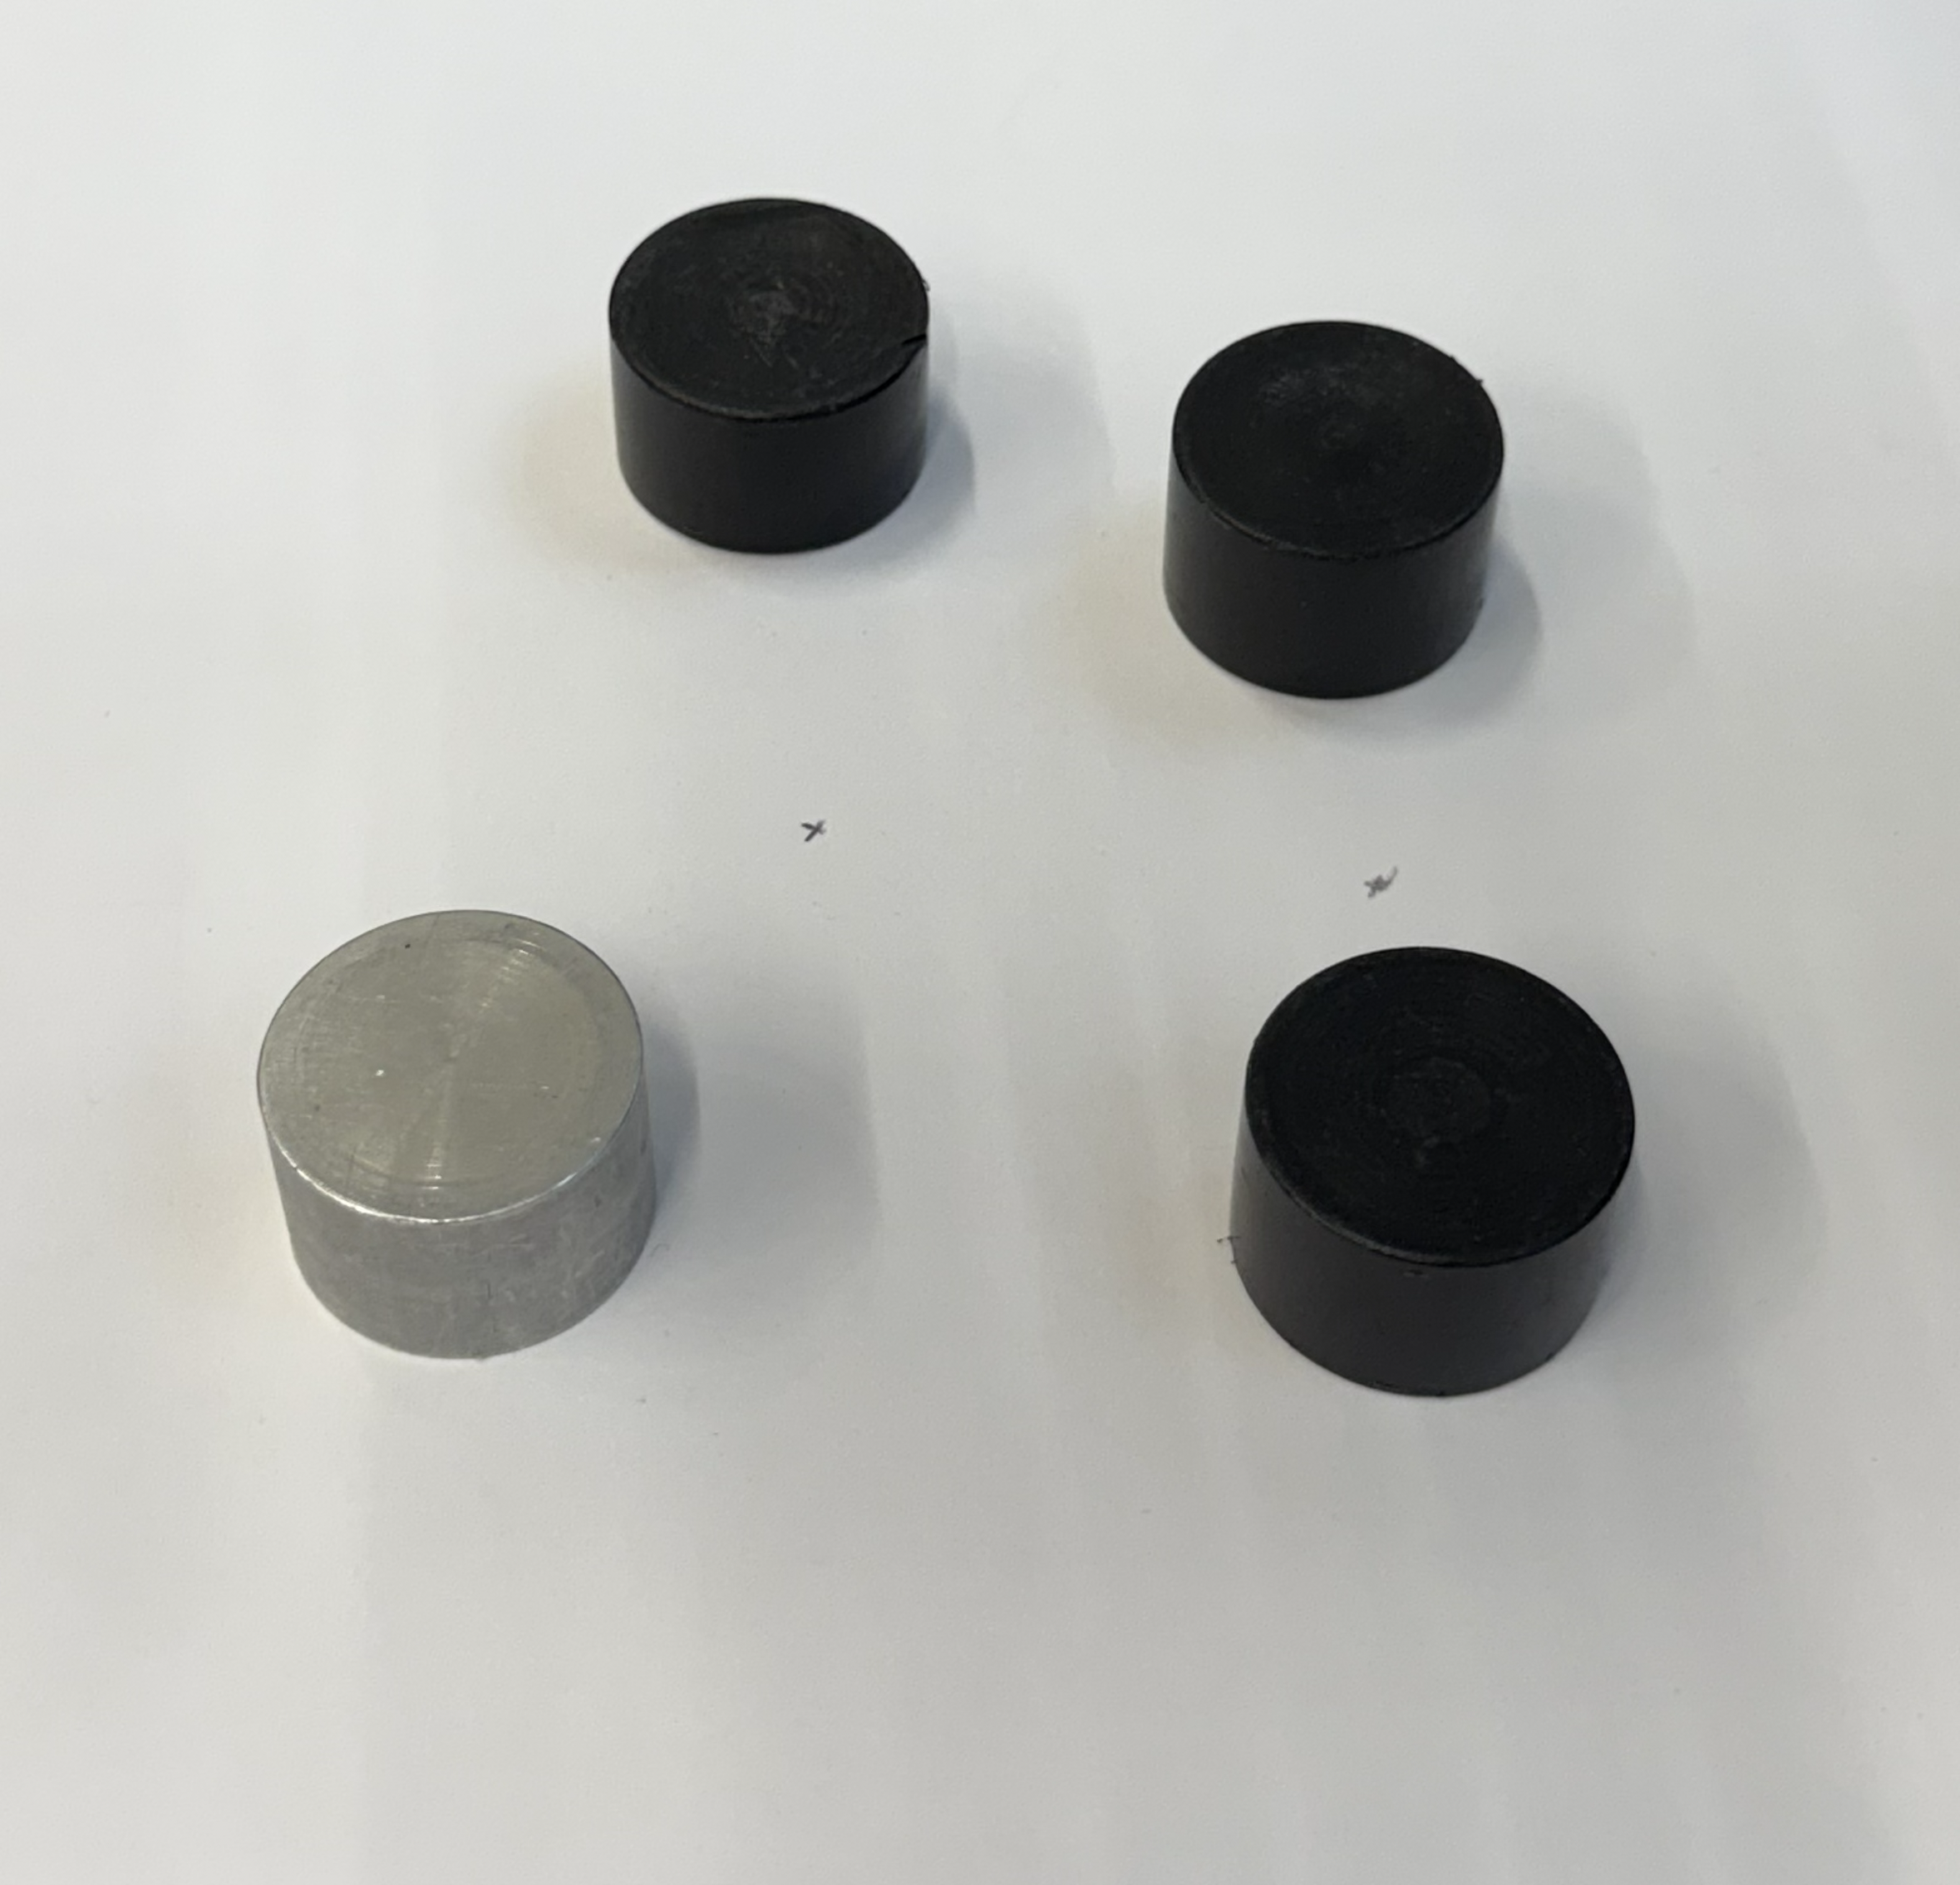
\includegraphics[width=\textwidth]{figures/Messexperiment}
		\caption{Objektanordnung}
		\label{fig:objektanordung}
	\end{subfigure}
	\hfill % Sorgt für gleichmäßigen Abstand zwischen den Bildern
	% Zweites Bild (TikZ)
	\begin{subfigure}[b]{0.45\textwidth}
		\centering
		\begin{tikzpicture}[
			box/.style={draw, minimum width=2.5cm, minimum height=0.8cm, align=center},
			greenbox/.style={box, fill=green!20},
			yellowbox/.style={box, fill=yellow!30},
			graybox/.style={box, fill=gray!30},
			node distance=0.45cm % Abstand zwischen den Boxen
			]
			
			% 5 grüne Boxen untereinander
			\node[graybox] (G0) {Objekt-ID: X-, Y-, Z-, Roll, Pitch};
			\node[greenbox, below=of G0] (G1) {Objekt 1: -42, 291, 6, -90, -8};
			\node[greenbox, below=of G1] (G2) {Objekt 2: -37, 374, 6, -90, -5};
			\node[greenbox, below=of G2] (G3) {Objekt 3: 36, 295, 6, -90, 6};
			\node[greenbox, below=of G3] (G4) {Objekt 4: 55, 346, 6, -90, 9};	
		\end{tikzpicture}
		\caption{Koordinaten im Messexperiment}
		\label{fig:koordinaten}
	\end{subfigure}
	\caption{Messexperiment zur Evaluation der Sortierperformance}
	\label{fig:messexperiment}
\end{figure}
Die Geschwindigkeit des Roboters wird per Befehl \textbf{SP} fest auf Stufe 5 (0-9 Stufen) gesetzt. Sowohl die maximalen als auch die eingestellten Geschwindigkeiten der einzelnen Achsen lassen sich aus Tabelle \ref{tab:geschwindikeiten_movemaster} entnehmen und sind für die spätere Betrachtung der inversen Kinematik des Movemaster EX RV-M1 relevant.

\begin{table}[h!]
	\renewcommand{\arraystretch}{1.2} % Etwas mehr Zeilenabstand
	\begin{tabular}{|c|c|c|}
		\hline
		\textbf{Achse} & \textbf{maximale Geschwindigkeit} & \textbf{SP5-Geschwindigkeit} \\ \hline
		Joint 1 & 120 °/sec & 29,64 °/sec \\ \hline
		Joint 2 & 72 °/sec & 17,78 °/sec\\ \hline
		Joint 3 & 109 °/sec & 26,92 °/sec \\ \hline
		Joint 4 & 100 °/sec & 24,7 °/sec\\ \hline
		Joint 5 & 163 °/sec & 40,26 °/sec\\ \hline
	\end{tabular}
	\caption{maximale bzw. SF5-Gelenkgeschwindigkeiten nach \cite[APP-52, 1-7]{rvm1manual}}
	\label{tab:geschwindikeiten_movemaster}	
\end{table}
\newpage Das Ziel, alle Objekte jeweils in einen leeren Magazinplatz zu sortieren, kann in vier Objektsortierungssequenzen und zwei Sequenzen für die Start-/Endposition eingeteilt werden. Dabei enthält jede Objektsortierungssequenz Fahr- und Greifbefehle - ersichtlich in Abbildung \ref{fig: objektsequenz}.
\begin{figure}[h!]
	\centering
	\begin{tikzpicture}[
		% Definition der Stile
		fahr/.style={rectangle, draw=blue!70, fill=blue!10, minimum height=0.8cm, minimum width=1.5cm, align=center, font=\tiny\sffamily},
		greif/.style={rectangle, draw=orange!80, fill=yellow!30, minimum height=0.8cm, minimum width=1.0cm, align=center, font=\tiny\sffamily},
		arrow/.style={-{Stealth[scale=1.2]}}
		]
		
		% --- Sequenz der Boxen ---
		\node[fahr] (B0) {Z-Offset\\Objekt\\anfahren};
		\node[fahr, right=0.2cm of B0] (B1) {Objekt\\anfahren};
		\node[greif, right=0.2cm of B1] (B2) {Greifer\\schließen};
		\node[fahr, right=0.2cm of B2] (B3) {Z-Offset\\Objekt\\anfahren};
		\node[fahr, right=0.2cm of B3] (B4) {Z-Offset\\Magazin\\anfahren};
		\node[fahr, right=0.2cm of B4] (B5) {Magazin-\\platz\\anfahren};
		\node[greif, right=0.2cm of B5] (B6) {Greifer\\öffnen};
		\node[fahr, right=0.2cm of B6] (B7) {Z-Offset\\Magazin\\anfahren};
		
		% --- Zeitstrahl ---
		\draw[arrow, thick] ($(B0.south west)-(0,0.5)$) -- ($(B7.south east)+(0,-0.5)$) node[right, font=\tiny] {Zeit $T_{objekt}$};
		
		% Verbindungsline zur Verdeutlichung der Sequenz
		\draw[dashed, gray] (B1.south) -- ++(0,-0.3);
		\draw[dashed, gray] (B7.south) -- ++(0,-0.3);
		
	\end{tikzpicture}
	\caption{Befehle innerhalb einer Objektsortierungssequenz}
	\label{fig: objektsequenz}
\end{figure}
\newline Die theoretische Gesamtverfahrzeit die der Roboter für die Sortierung aller vier Objekte benötigt, setzt sich somit zusammen aus: 
\begin{itemize}
	\item Zeit zum Erreichen der Startposition
	\item $4*T_{Objekt}$ aus \ref{fig: objektsequenz}
	\item Zeit zum Erreichen der Endposition
\end{itemize}

\newpage

\subsubsection{Praktische Limitation - Laufzeitmessung mit Simulationsexperiment}
Um die praktische Limitation der bisherigen Architektur sinnvoll beurteilen zu können, wird zunächst die theoretisch benötigte Laufzeit mit Gleichung \ref{Summation Befehlsausführungszeiten mit eingesetzten Zeiten} ermittelt.
\begin{equation*}
	T_{s} = \sum_{i=1}^{n} \sum_{j=1}^{k} (T_{senden, i, j} + T_{schlafen, i, j})
\end{equation*}
Betrachtet man den Programmcode der Klasse \textit{Roboter.cs}, so fällt auf, dass jeder Sendevorgang ($T_{senden,i,j}$) mit einem Thread.Sleep() von 800ms beaufschlagt wird. Dies geschieht, um sicherzugehen, dass der interne
\begin{table}[h!]
	\centering
	\renewcommand{\arraystretch}{1.2}
	\begin{tabular}{|c|c|c|}
		\hline
		 \textbf{Beschreibung} & \textbf{Thread.Sleep() [ms]} & $T_{schlafen,i,j}$ \\ \hline
		Fahrt auf Objekt Z-Offset  & 3000 & $T_{schlafen,i,1}$ \\ \hline
		Absenken auf Objektposition & 3000 & $T_{schlafen,i,2}$ \\ \hline
		Objekt greifen & 500 & $T_{schlafen,i,3}$ \\ \hline
		Anheben auf Objekt Z-Offset & 2000 & $T_{schlafen,i,4}$ \\ \hline
		Fahren auf Magazin Z-Offset & 5000 & $T_{schlafen,i,5}$ \\ \hline
		Absenken auf Magazinposition & 1000 & $T_{schlafen,i,6}$\\ \hline
		Loslassen des Objekts & 1000 & $T_{schlafen,i,7}$ \\ \hline
		Anheben auf Magazin Z-Offset & 1000 & $T_{schlafen,i,8}$ \\ \hline
		\textit{Anheben auf Magazin Z-Offset} & 1000 & $T_{schlafen,i,9}$ \\ \hline
	\end{tabular}
	\caption{Tabellarische Übersicht der Thread.Sleep()-Verzögerung pro Objektsequenz}
	\label{tab:thread.sleep()-zeiten}
\end{table} 
\newline Setzt man nun die ermittelten statischen Werte aus Tabelle \ref{tab:thread.sleep()-zeiten}, die Wartezeiten bei jedem Senden sowie die Zeit für Start- und Endposition in die Gleichung für die Gesamtdauer $T_{S}$ ein:
\begin{equation}
	T_{S} = 	T_{s} = 2*(1800ms) \sum_{i=1}^{4} \sum_{j=1}^{9} (T_{senden, i, j} + T_{schlafen, i, j})
\end{equation}
so erhält man eine berechnete Gesamtdauer von 



\begin{table}[h!]
	\renewcommand{\arraystretch}{1.2} % Etwas mehr Zeilenabstand
	\begin{tabular}{|c|c|c|}
		\hline
		\textbf{Objekt-ID} & \textbf{Theoretische Zeit $T_S$ [s]} & \textbf{Gemessene Zeit $T_{mess}$ [s]} \\ \hline
		Startposition & 1,8 & 24,97 \\ \hline
		Objekt 1 & 17,5 & 24,97 \\ \hline
		Objekt 2 & 17,5 & 24,91 \\ \hline
		Objekt 3 & 17,5 & 24,95 \\ \hline
		Objekt 4 & 17,5 & 24,89 \\ \hline
		Endposition & 1,8 & 24,97 \\ \hline
		\textbf{Mittelwert} & \textbf{17,5} & \textbf{24,93} \\ \hline
		\textbf{$T_{S}$} & \textbf{70} & \textbf{103,73} \\ \hline
	\end{tabular}
	\caption{Vergleich der theoretischen Laufzeit $T_S$ mit den gemessenen Werten $T_{mess}$}
	\label{tab:laufzeitanalyse_ist}
\end{table}


\newpage

%%
\chapter{Roboter-Befehlspipeline}
\label{Roboter-Befehlspipeline}
Dieses Kapitel detailliert die Konzeptionierung und Implementierung einer Steuerungslogik für den Mitsubishi Movemaster EX RV-M1, welche auf dem Prinzip einer Warteschlange basiert. 
\newpage

%%
\chapter{Implementation der Erweiterungen}
Warteschlange, Safety, Punktwolkenspeicherung, ...

\newpage

%%
\chapter{Fazit \& Ausblick}
\label{kap:Fazit und Ausblick}
Im Rahmen dieser Studienarbeit konnte erfolgreich die methodische und technische Grundlage für die Transformation des vorhandenen Robotersystems - bestehend aus dem EX RV-M1 und einem Vision-System (2D \& 3D-ToF) - hin zu einem limitiert kollaborativen und dynamischen System gelegt werden.
\\
\\Zunächst wurden durch eine IST-Analyse die konkreten Limitationen der synchronen Softwarearchitektur, insbesondere die blockierenden Wartezeiten durch die Verwendung von Thread.Sleep()-Befehlen, quantitativ aufgezeigt. Auf Basis dieser Erkenntnisse wurde eine asynchrone Befehlsstruktur konzipiert und implementiert. Diese verwendet moderne .NET-Prinzipien (TPL und TAP) und eine prädiktive Zeitberechnung mittels inverser Kinematik, um die Laufzeit des Systems an die physisch auszuführenden Bewegung anzupassen. Diese Umstellung bietet weitere Optimierungspotenziale und Testfälle, welche in nachfolgenden Arbeiten umgesetzt werden können. Dazu zählen:
\begin{itemize}
	\item Weitere Optimierung der Laufzeit durch Messung der real benötigten Zeit für das Senden von Befehlen sowie Öffnen/Schließen des Greifers
	\item Aufbrechen der MP-Befehle über Trajektoriensegmentierung um ein schnelleres Stoppen der Pipeline nach jedem gefahrenen Segment zu realisieren (vgl. Konzept in Studienarbeit T3100 Adrian Sommer \& Luis Thiel)
	\item Grenzfallbetrachtung: Tests mit verschiedenen Objekten und Orientierungen - Zuverlässigkeit und Reproduzierbarkeit evaluieren
\end{itemize}
Des Weiteren konnte eine aktive Detektion von menschlichen Händen mithilfe der 2D-Kamera umgesetzt werden. Hierzu kommt die Machine-Learning-Methode \textit{Haar Cascade Classifier} zum Einsatz. Dabei handelt es sich um einen vortrainierten Datensatz, welcher es ermöglicht, einen fest definierten Arbeitsbereich zu überwachen und diesen nach Merkmalen zu filtern, welche einer Hand entsprechen. Die finale Implementation wurde erfolgreich mittels einer Testreihe validiert, in welcher auch ein Ignorieren der für den Roboter relevanten Objekte gezeigt wurde.\\
\\Aufbauend auf dieser Studienarbeit ergeben sich für die Zukunft Weiterentwicklungspotenziale wie z.B. die Untersuchung von KI-basierten Safety-Ansätzen oder die Implemenation eines externen Sensor/CPU-System um einen hardwareseitigen Not-Halt in die Steuerung zu implementieren.

\newpage

%%
%%%%%%%%%%%%%%%%%%%%%%%%%%%%%%%%%%%%%%%%%%%%%%%%%%%%%%%%%%%%%%%%%%%%
% Anhang
%%%%%%%%%%%%%%%%%%%%%%%%%%%%%%%%%%%%%%%%%%%%%%%%%%%%%%%%%%%%%%%%%%%%

\chapter{Anhang}
\label{Anhang}

\newpage

\pagenumbering{roman}
\setcounter{page}{7}
%%%%%%%%%%%%%%%%%%%%%%%%%%%%%%%%%%%%%%%%%%%%%%%%%%%%%%%%%%%%%%%%%%%%%%%%%%%%%
%%% Bibliographie
%%%%%%%%%%%%%%%%%%%%%%%%%%%%%%%%%%%%%%%%%%%%%%%%%%%%%%%%%%%%%%%%%%%%%%%%%%%%%

\addcontentsline{toc}{chapter}{Literaturverzeichnis}

\bibliographystyle{IEEEtran}
\bibliography{mylit}
%% Obige Anweisung legt fest, dass BibTeX-Datei `mylit.bib' verwendet
%% wird. Hier koennen mehrere Dateinamen mit Kommata getrennt aufgelistet
%% werden.

%%%%%%%%%%%%%%%%%%%%%%%%%%%%%%%%%%%%%%%%%%%%%%%%%%%%%%%%%%%%%%%%%%%%%%%%%%%%%
%%% Abk"urzungsverzeichnis
%%%%%%%%%%%%%%%%%%%%%%%%%%%%%%%%%%%%%%%%%%%%%%%%%%%%%%%%%%%%%%%%%%%%%%%%%%%%%

\addcontentsline{toc}{chapter}{Abk"urzungsverzeichnis}
\chapter*{Abk"urzungsverzeichnis}
\markboth{ABKÜRZUNGSVERZEICHNIS}{ABKÜRZUNGSVERZEICHNIS}
\begin{tabbing}
	
	% Definiere den Abstand: Hier 4cm für die Abkürzung, dann kommt der Rest
	xxxxxxxxxxxxxx \= \kill 
	
	
	CLR \> Common Language Runtime
	\\CMOS \> Complementary Metal-Oxide-Semiconducto
	\\Cobot \> Collaborative Robot
	\\CTS \> Clear to Send 
	\\DFT \> Diskrete Fouriertransformation
	\\DH \> Denavit Hartenberg
	\\DIN \> Deutsches Institut für Normung
	\\DLL \> Dynamic Link Library
	\\DSR \> Data Set Ready 
	\\DTR \> Data Terminal Ready
	\\DU \> Drive Unit
	\\EN \> Europäische Norm
	\\ER \> Error Read
	\\FG \> Frame Ground
	\\FOV \> Field of View
	\\fps \> frames per second (Bilder pro Sekunde)
	\\IPK \> Institut für Produktionsanlagen und Konstruktionstechnik
	\\ISO \> International Organization for Standardization
	\\JSON \> JavaScript Object Notation
	\\KI \> Künstliche Intelligenz
	\\LED \> Leuchtdiode
	\\LIDAR \> Light Detection and Ranging
	\\MC \> Move Continuous 
	\\ML \> Maschinelles Lernen
	\\MO \> Move
	\\ms \> Millisekunde
	\\Mutex \> Mutual Exclusions
	\\MVC \> Model View Controller
	\\NC \> Not Connected 
	\\P/Invoke \> Platform Invocation Services 
	\\PCL \> Point Cloud Library 
	\\PL \> Performance Level 
	\\RANSAC \> Random Sample Consensus Algorithmus
	\\RXD \> Receive Data
	\\ROR \> Radius Outlier Removal 
	\\RS-232 \> Recommended Standard 232
	\\SCARA \> Selective Compliance Assembly Robot Arm 
	\\SOR \> Statistical Outlier Removal 
	\\SP \> Speed  
	\\SSM \> Speed and Separation Monitoring 
	\\TCP \> Tool Center Point 
	\\TCP/IP \> Transmission Control Protocol/Internet Protocol 
	\\ToF \> Time of Flight
	\\TXD \> Transmit Data
	\\WH \> Where
	\\2D \> Zweidimensional  
	\\3D \> Dreidimensional
\end{tabbing}

\newpage
%%%%%%%%%%%%%%%%%%%%%%%%%%%%%%%%%%%%%%%%%%%%%%%%%%%%%%%%%%%%%%%%%%%%%%%%%%%%%
%%% Abbildungsverzeichnis
%%%%%%%%%%%%%%%%%%%%%%%%%%%%%%%%%%%%%%%%%%%%%%%%%%%%%%%%%%%%%%%%%%%%%%%%%%%%%

\renewcommand{\baselinestretch}{1.3}
\small\normalsize

\addcontentsline{toc}{chapter}{Abbildungsverzeichnis}
\listoffigures

\renewcommand{\baselinestretch}{1}
\small\normalsize

\newpage

%%%%%%%%%%%%%%%%%%%%%%%%%%%%%%%%%%%%%%%%%%%%%%%%%%%%%%%%%%%%%%%%%%%%%%%%%%%%%
%%% Tabellenverzeichnis
%%%%%%%%%%%%%%%%%%%%%%%%%%%%%%%%%%%%%%%%%%%%%%%%%%%%%%%%%%%%%%%%%%%%%%%%%%%%%

%\renewcommand{\baselinestretch}{1.3}
%\small\normalsize

%\addcontentsline{toc}{chapter}{Tabellenverzeichnis}
%\listoftables

%\renewcommand{\baselinestretch}{1}
%\small\normalsize

%\newpage

%%%%%%%%%%%%%%%%%%%%%%%%%%%%%%%%%%%%%%%%%%%%%%%%%%%%%%%%%%%%%%%%%%%%%%%%%%%%%
%%% Anhang
%%%%%%%%%%%%%%%%%%%%%%%%%%%%%%%%%%%%%%%%%%%%%%%%%%%%%%%%%%%%%%%%%%%%%%%%%%%%%
\clearpage % Beendet das vorherige Kapitel sauber
\newpage
\addcontentsline{toc}{chapter}{Erklärungen zur Arbeit und Hilfsmitteln}
\chapter*{Erklärungen zur Arbeit und Hilfsmitteln}
\markboth{ERKLÄRUNGEN}{ERKLÄRUNGEN}

\subsection*{Verwendete Hilfsmittel}
Für die Erstellung dieser Studienarbeit wurden folgende Tools eingesetzt:
\begin{itemize}
	\item \textbf{Hardware:} SICK Visionary-T Mini-CX, Mitsubishi Movemaster EX-RV M1, uEye Industriekamera
	\item \textbf{Software:} OpenCV Bibliothek, Visual Studio (C++ und \csharp), RoboETH, drawIO (Erstellung von Grafiken), texStudio, uEye-Cockpit und IDS Kameramanager, GitHub (Kollaboratives Arbeiten und Versionsverwaltung der LaTeX-Vorlage).
\end{itemize}
\subsubsection*{KI-Tools und relevanter Einsatzbereich}
\label{KI-Tools und relevanter Einsatzbereich}
Dies erfolgt im Einklang mit der entsprechenden Verordnung der DHBW \href{https://www.dhbw.de/fileadmin/user_upload/Dokumente/Dokumente_fuer_Studierende/191212_Leitlinien_Praxismodule_Studien_Bachelorarbeiten.pdf}{(Weblink)}.
\begin{table}[H]
	\centering
	\begin{tabular}{|p{3cm}|p{6cm}|p{2.5cm}|}
		\hline
		\textbf{Tool} & \textbf{Art der Nutzung} & \textbf{Abschnitt} \\ \hline
		{Google Gemini AI Student Pro License} & {Formatierung von LaTeX-Code, Erstellung von Blankovorlagen für Tabellen und Listen} & {gesamte Arbeit} \\ \hline
		{Google Gemini AI Student Pro License: Deep Search-Feature} & {Tiefgreifende Analyse des Datenblatts des Movemaster EX RV-M1: Finden von Abschlusszeichen im RS232-String, Pin-Belegung für Hardwaregestütztes Acknowledgement über RS232, Physikalische Signalanalyse für die Implementierung einer Flow-Control; Ergebnis der "Deep Search" kann jederzeit als PDF-Dokument bereitgestellt werden} & {4.3.2} \\ \hline
		{DeepL AI Übersetzer} & {Formulierung des englischsprachigen Abstracts} & {Abstract} \\ \hline
	\end{tabular}
\end{table}
\newpage
\subsection*{Aufteilung der Kapitel}
Die Erstellung der vorliegenden Studienarbeit erfolgte in gemeinsamer Kooperation. In der folgenden Tabelle ist dokumentiert, welcher Autor die primäre Urheberschaft für die jeweiligen Kapitel bzw. Abschnitte trägt:

\vspace{0.5cm}
\renewcommand{\arraystretch}{1.5} %Felder dieser Tabelle auf 1.5x 
\noindent
\begin{tabularx}{\textwidth}{|X|l|l|}
	\hline
	\textbf{Kapitel / Abschnitt} & \textbf{Kapitelnummer} & \textbf{Autor} \\ \hline
	Einleitung                           & \ref{Einleitung} & Gemeinsame Bearbeitung \\ \hline
	Robotik                              & \ref{Robotik} & \autor \\ \hline
	Industrielle Bildverarbeitung        & \ref{Bildverarbeitung} & \autorzwei \\ \hline
	Grundlagen der Informatik            & \ref{Grundlagen der Informatik} & \autor \\ \hline
	Hardware                             & \ref{Ausgangslage: Hardware} & \autor \\ \hline
	Software                             & \ref{Ausgangslage: Software} & \autorzwei \\ \hline
	Messreihe							 & \ref{Messreihe} & \autor \\ \hline
	Optimierung der Softwarestruktur	 & \ref{Optimierung der Softwarestruktur} & \autor \\ \hline
	Optimierung der Bildgewinnung   	 & \ref{Optimierung der Bildgewinnung} & \autor \\ \hline
	Optimierung und Verbesserungsmöglichkeiten an der Software & \ref{Optimierung und Verbesserungsmöglichkeiten an der Software} & \autorzwei \\ \hline
	Normative Anforderungen 		     & \ref{Normative Anforderungen und Grenzen des RV-M1} & Gemeinsame Bearbeitung \\ \hline
	Umsetzbare Sicherheitsanforderungen	 & \ref{Umsetzbare Sicherheitsmerkmale} & Gemeinsame Bearbeitung \\ \hline
	Ansatz Geschwindigkeits- und Abstandsüberwachung & \ref{Ansatz Geschwindigkeits- und Abstandsüberwachung} & \autorzwei \\ \hline
	Fazit und Ausblick                   & \ref{Fazit und Ausblick} & Gemeinsame Bearbeitung \\ \hline
\end{tabularx}
\newpage
Hiermit bestätigen wir, \autor{} und \autorzwei, dass die oben gemachten Angaben der Wahrheit entsprechen.
\vspace{2cm} % Abstand zum Text
% --- Block für Autor 1 (Luis) ---
\noindent
\begin{tabular}{@{}p{6cm}p{7cm}@{}}
	% Ort mit Datum & Unterschrift (mit raisebox nach unten geschoben)
	\vspace{1.1cm} Horb, den \today & 
	% ÄNDERUNG: raisebox schiebt das Bild tiefer.
	% Spiel mit dem Wert "-1.8cm", bis es perfekt auf der Linie sitzt.
	\raisebox{-1.8cm}[0pt][0pt]{
\includegraphics[height=1.5cm, keepaspectratio]{figures/L_Signature.png}} 
	\\[-0.5ex] 
	
	% Die Linien
	\rule{5.5cm}{0.4pt} & \rule{6.5cm}{0.4pt} \\
	
	% Beschriftung
	\footnotesize Ort, Datum & \footnotesize Unterschrift (\autor)
\end{tabular}

\vspace{0.75cm} % Abstand zwischen den Autoren

% --- Block für Autor 2 ---
\noindent
\begin{tabular}{@{}p{6cm}p{7cm}@{}}
	\vspace{1.1cm} Horb, den \today & 
	% ÄNDERUNG: Auch hier raisebox nutzen
	\raisebox{-1.8cm}[0pt][0pt]{
\includegraphics[height=1.5cm, keepaspectratio]{figures/A_Signature.png}} 
	\\[-0.5ex]
	
	\rule{5.5cm}{0.4pt} & \rule{6.5cm}{0.4pt} \\
	
	\footnotesize Ort, Datum & \footnotesize Unterschrift (\autorzwei)
\end{tabular}
\clearpage % Beendet das vorherige Kapitel sauber
\chapter*{Anhang}

\section*{Inhalt des digitalen Anhangs}
\label{Inhalt des digitalen Anhangs}
\begin{itemize}
	\item Anleitung zur Programmaufsetzung (Luis Thiel)
	\item gesamter LaTeX-Ordner
\end{itemize}
\newpage

%%%%%%%%%%%%%%%%%%%%%%%%%%%%%%%%%%%%%%%%%%%%%%%%%%%%%%%%%%%%%%%%%%%%%%%%%%%%%
%%% Ende
%%%%%%%%%%%%%%%%%%%%%%%%%%%%%%%%%%%%%%%%%%%%%%%%%%%%%%%%%%%%%%%%%%%%%%%%%%%%%

\end{document}

